% Om Tank, 18-645 mid-project talk: the 3x3 stride-1 convolution microkernel (7 slides, ~5 min).
% Overleaf: upload the zip, compile with pdfLaTeX. Figures are in figs/ (from results/ on branch om/conv3x3-s1).
% Every % of peak assumes the core runs at 3.4 GHz (max turbo), as in Assignment 2.
% Speaker notes: \note{} after each frame; to show them, add \setbeameroption{show notes on second screen=right}.
\documentclass[aspectratio=169,10pt]{beamer}
\usepackage{booktabs}
\usepackage{pgfplots}
\pgfplotsset{compat=1.17}
\usepackage{tikz}

% ---- palette (same as the figures and the pptx)
\definecolor{ink}{HTML}{1B2630}
\definecolor{muted}{HTML}{5A6875}
\definecolor{teal}{HTML}{0C6A87}
\definecolor{tealsoft}{HTML}{D7EAF0}
\definecolor{amber}{HTML}{B7731A}
\definecolor{ambersoft}{HTML}{F5E6CF}
\definecolor{navy}{HTML}{0E2F3B}
\definecolor{soft}{HTML}{EEF2F4}
\definecolor{grey}{HTML}{6B7782}

\usetheme{default}
\setbeamertemplate{navigation symbols}{}
\setbeamercolor{normal text}{fg=ink}
\setbeamercolor{frametitle}{fg=ink}
\setbeamerfont{frametitle}{size=\LARGE,series=\bfseries}
\setbeamercolor{block title}{fg=ink,bg=soft}
\setbeamercolor{block body}{fg=muted,bg=soft}
\setbeamercolor{block title alerted}{fg=teal,bg=tealsoft}
\setbeamercolor{block body alerted}{fg=muted,bg=tealsoft}
\setbeamertemplate{blocks}[rounded]
\setbeamertemplate{itemize item}{\color{teal}$\bullet$}
\setbeamertemplate{footline}{%
  \hspace{1.2em}{\color{muted}\scriptsize Om Tank $\cdot$ 18-645 $\cdot$ 3$\times$3 stride-1 kernel $\cdot$ ece028 (Xeon E5-2640 v4)}%
  \hfill{\color{muted}\scriptsize\insertframenumber}\hspace{1.2em}\vspace{0.8em}}

\newcommand{\stat}[3][teal]{{\color{#1}\fontsize{26}{28}\selectfont\bfseries #2}\\[2pt]{\small\color{muted}#3}}
\newcommand{\term}[3][block]{\begin{#1}{\texttt{#2}}\footnotesize #3\end{#1}}

\title{The 3$\times$3 stride-1 convolution kernel}
\author{Om Tank}

\begin{document}

% ------------------------------------------------------------------ 1. intro
{\setbeamercolor{background canvas}{bg=navy}\setbeamertemplate{footline}{}
\begin{frame}
  \vspace{1.2em}
  {\color{white}\fontsize{30}{34}\selectfont\bfseries The 3$\times$3 stride-1\\[4pt] convolution kernel\par}
  \vspace{0.6em}
  {\color{tealsoft}\large Om Tank $\cdot$ YOLOv8n on one Broadwell core, built like the Assignment 2 kernel\par}
  \vspace{2.2em}
  \begin{columns}[T]
    \begin{column}{0.23\textwidth}\stat[white]{32}{\color{tealsoft}layers: C2f bottlenecks + Detect head}\end{column}
    \begin{column}{0.23\textwidth}\stat[white]{66\%}{\color{tealsoft}of YOLOv8n's 8.74 GFLOP}\end{column}
    \begin{column}{0.23\textwidth}\stat[white]{94\%}{\color{tealsoft}of peak: best microkernel alone}\end{column}
    \begin{column}{0.23\textwidth}\stat[white]{84\%}{\color{tealsoft}of peak across all 32 real layers}\end{column}
  \end{columns}
\end{frame}}
\note{My kernel is the 3x3 stride-1 convolution: 32 layers, the C2f bottlenecks and the Detect head, two thirds of YOLOv8n's work.
The story: it is the Assignment 2 kernel, I followed the same four steps, and the measurements chose the tile.
Best microkernel alone: 94\% of the 32 FLOPs/cycle peak; inside all 32 real layers: 84\%. All percentages assume the core runs at 3.4 GHz, as in Assignment 2.}

% ------------------------------------------------------------------ 2. same as A2
\begin{frame}{It is the Assignment 2 kernel, with floats}
  \begin{columns}[T]
    \begin{column}{0.57\textwidth}
      \resizebox{\linewidth}{!}{%
      \begin{tabular}{@{}lll@{}}
        \toprule
        & \textbf{Assignment 2} & \textbf{Stride-1 microkernel} \\ \midrule
        $m$ (broadcast)   & 5 rows of A         & 5 output pixels \\
        $n$ (vector loads) & $8 = 2\times4$ doubles & 16 channels $= 2\times8$ floats \\
        $k$ (reduction)   & 32 to 512           & $C\times9$ (144 to 2304) \\
        Accumulators      & 10                  & 10 (2$\times$5) or 12 (2$\times$6) \\
        Registers         & 13 of 16            & 13 or 15 of 16 \\
        Peak per core     & 16 FLOPs/cycle      & 32 FLOPs/cycle \\ \bottomrule
      \end{tabular}}
      \vspace{1em}

      {\color{muted}Same Broadwell core: 2 FMA units $\times$ 8 lanes $\times$ 2 FLOPs $=$ 32 FLOPs/cycle.
      Latency 5 $\times$ throughput 2 $=$ 10 chains in flight.}
    \end{column}
    \begin{column}{0.38\textwidth}
      \term{C}{input channels of the layer (16 to 256)}
      \term{k = C x 9}{multiply-adds per output: $C$ channels $\times$ the 9 taps of the 3$\times$3 filter (A2's $k$)}
      \term{accumulator}{one YMM register $=$ 8 outputs (8 channels of one pixel); one dependency chain}
      \term[alertblock]{tile 2x5 (10)}{outputs per call: 2 blocks of 8 channels $\times$ 5 pixels $=$ 80 outputs in 10 accumulators}
    \end{column}
  \end{columns}
\end{frame}
\note{Same machine as Assignment 2 and the same kernel. In A2, m was 5 rows of A broadcast, n was 8 doubles = 2 vectors of B.
Here m is 5 output pixels, n is 16 output channels = 2 vectors of 8 floats, and k is input channels times the 9 taps of the 3x3 filter.
10 accumulators, 13 registers, exactly the A2 budget. Peak is 32 FLOPs per cycle because floats give 8 lanes instead of 4.
10 accumulators is the minimum (5 x 2); the 2x6 tile uses 12, two chains of slack.}

% ------------------------------------------------------------------ 3. the tile as tensors
\begin{frame}{One kernel call = 80 outputs}
  \centering
  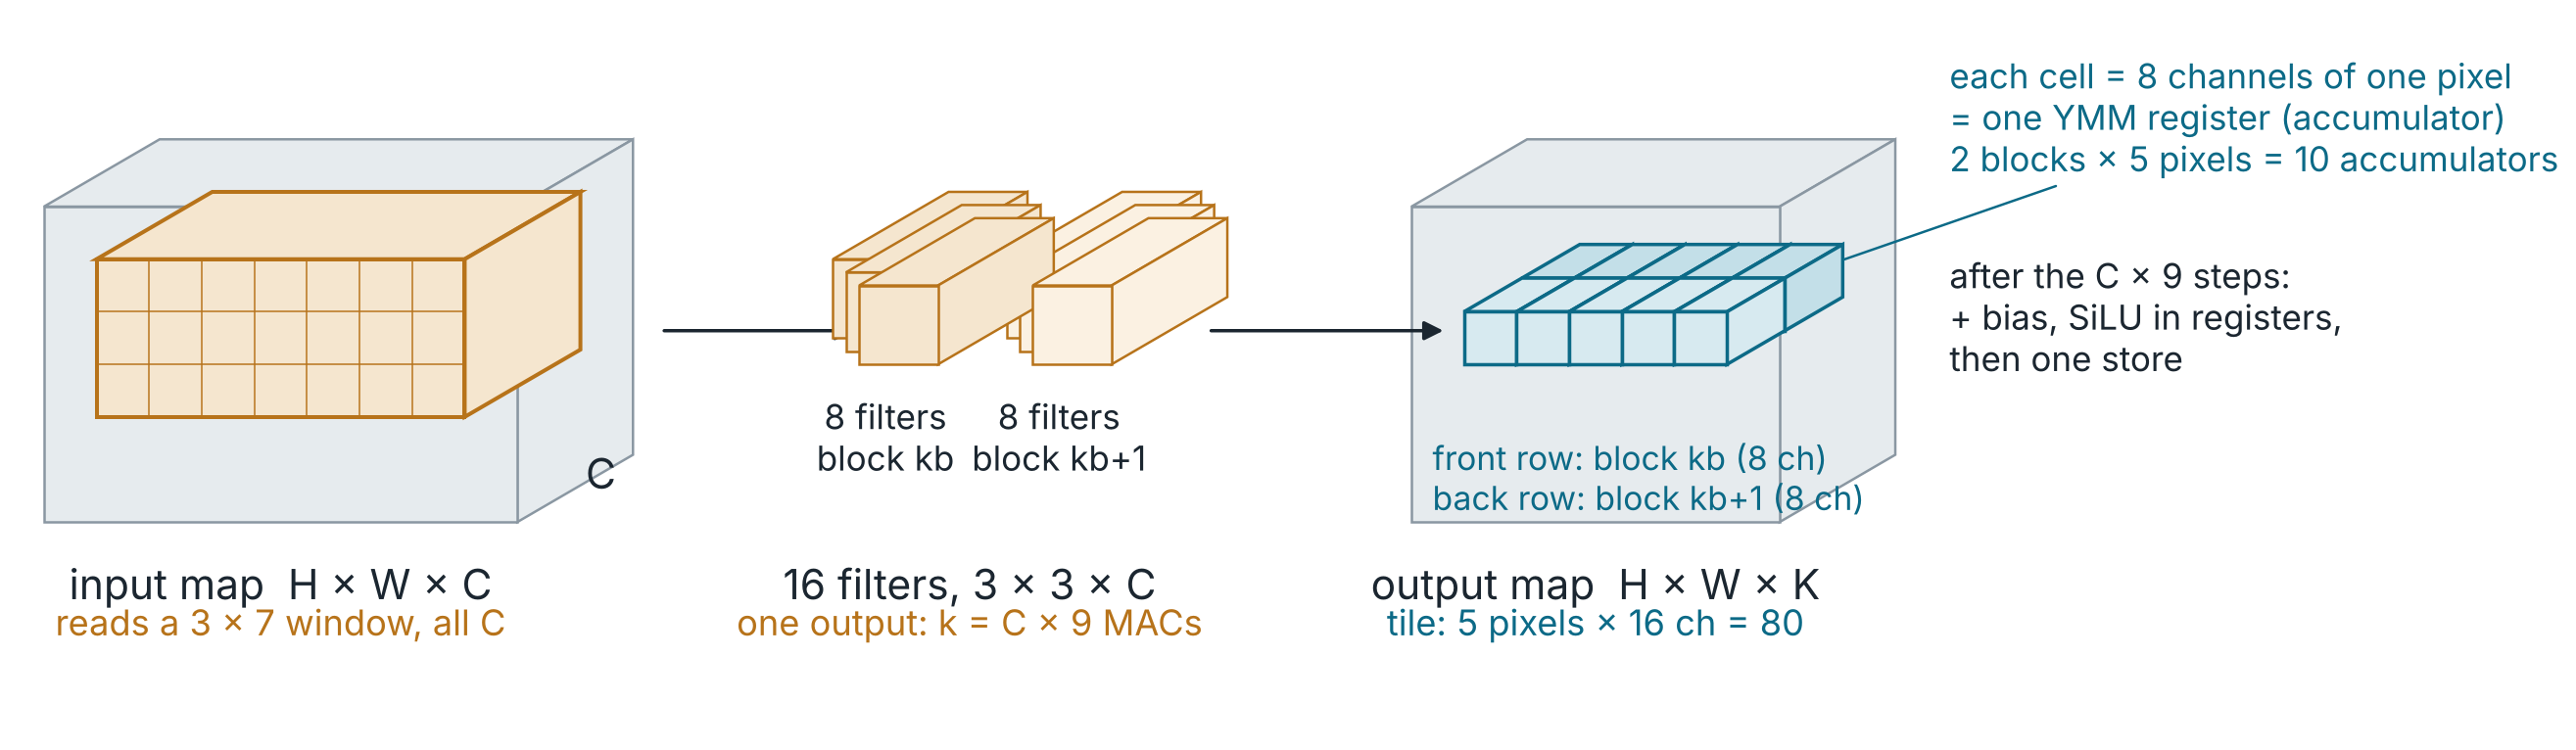
\includegraphics[width=0.95\textwidth]{figs/tile_tensors.png}

  \vspace{1em}
  \raggedright
  Per step (one input channel at one of the 9 taps): load 2 weight vectors, broadcast 5 inputs, 10 FMAs.
  Repeat $k = C\times9$ times, then bias, SiLU and one store per register.
\end{frame}
\note{One call computes the teal strip: one output row, 5 pixels wide, 16 output channels deep, 80 numbers.
Each cell is 8 channels of one pixel, exactly one YMM register, so the strip is 10 accumulators.
It reads a 3 by 7 window of the input across all C channels (5 pixels plus one on each side, 3 filter rows) and 16 filters of 3 by 3 by C.
Each step multiplies 2 weight vectors by 5 broadcast inputs, 10 FMAs, repeated k = C x 9 times, then bias, SiLU, store.}

% ------------------------------------------------------------------ 4. four steps
\begin{frame}{Four steps: ops $\rightarrow$ accumulators $\rightarrow$ tile $\rightarrow$ benchmark}
  \begin{columns}[T]
    \begin{column}{0.46\textwidth}
      \begin{enumerate}
        \setlength{\itemsep}{0.7em}
        \item \textbf{Independent ops.} {\small\color{muted}Every output is its own dot product of length $C\times9$: 102,400 in a 40$\times$40, 64-channel layer.}
        \item \textbf{Outputs in flight.} {\small\color{muted}Latency 5 $\times$ 2 FMA/cycle $=$ 10 accumulators $=$ 80 outputs; 1 accumulator runs at 10\% of peak.}
        \item \textbf{Kernel size.} {\small\color{muted}2$\times$5 tile: 10 acc $+$ 2 weights $+$ 1 broadcast $=$ 13 regs; 7 loads per 10 FMAs; 5 divides every width.}
        \item \textbf{Benchmark like A2.} {\small\color{muted}Microkernel alone, $k = 72$ to 4608, 3 runs, 2\,s warm-up, cycles at 3.4\,GHz, checked against a reference.}
      \end{enumerate}
    \end{column}
    \begin{column}{0.5\textwidth}
      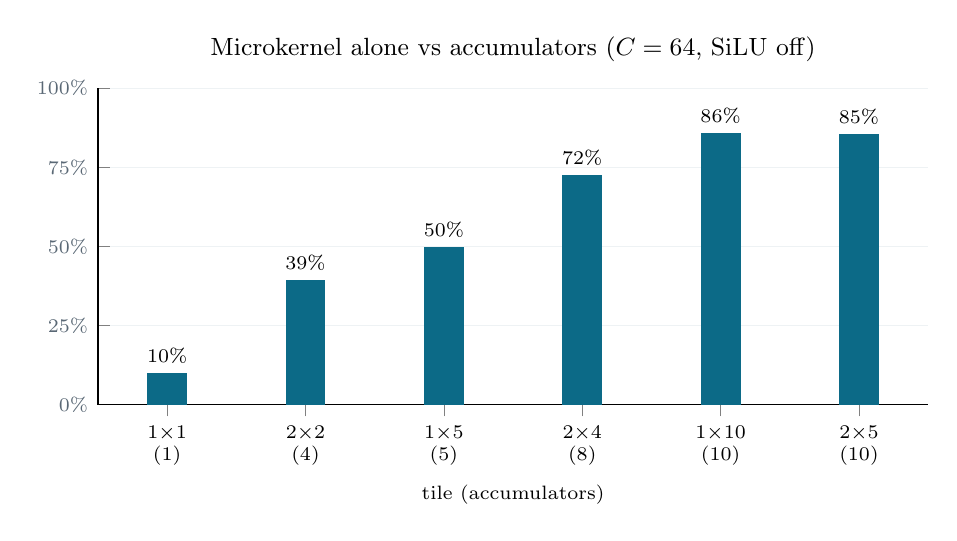
\begin{tikzpicture}
        \begin{axis}[width=\linewidth, height=5.6cm, ybar, bar width=14pt, ymin=0, ymax=100,
            ytick={0,25,50,75,100}, yticklabel={\pgfmathprintnumber{\tick}\%},
            symbolic x coords={1x1,2x2,1x5,2x4,1x10,2x5}, xtick=data,
            xticklabels={1$\times$1\\(1),2$\times$2\\(4),1$\times$5\\(5),2$\times$4\\(8),1$\times$10\\(10),2$\times$5\\(10)},
            x tick label style={font=\scriptsize, align=center}, y tick label style={font=\scriptsize, color=muted},
            nodes near coords={\pgfmathprintnumber[fixed,precision=0]{\pgfplotspointmeta}\%},
            nodes near coords style={font=\scriptsize}, axis lines*=left, ymajorgrids, grid style={color=soft},
            title={\small Microkernel alone vs accumulators ($C = 64$, SiLU off)}, xlabel={\scriptsize tile (accumulators)}]
          \addplot[fill=teal, draw=teal] coordinates {(1x1,9.9) (2x2,39.3) (1x5,49.6) (2x4,72.4) (1x10,85.8) (2x5,85.3)};
        \end{axis}
      \end{tikzpicture}
    \end{column}
  \end{columns}
\end{frame}
\note{Step 1: every output is an independent dot product; the only chain is the reduction.
Step 2: 5-cycle latency times 2 FMAs per cycle means 10 independent accumulators, 80 outputs in flight. The chart: 1 accumulator is 10\%, each adds about 10 points.
Step 3: 2x5 gives 10 accumulators in 13 registers, 7 loads per 10 FMAs, and 5 divides 160, 80, 40 and 20.
Step 4: benchmark the kernel alone exactly like Assignment 2.}

% ------------------------------------------------------------------ 5. design space
\begin{frame}{Same math, 50\% to 95\%: tile and register allocation}
  \begin{columns}[T]
    \begin{column}{0.8\textwidth}
      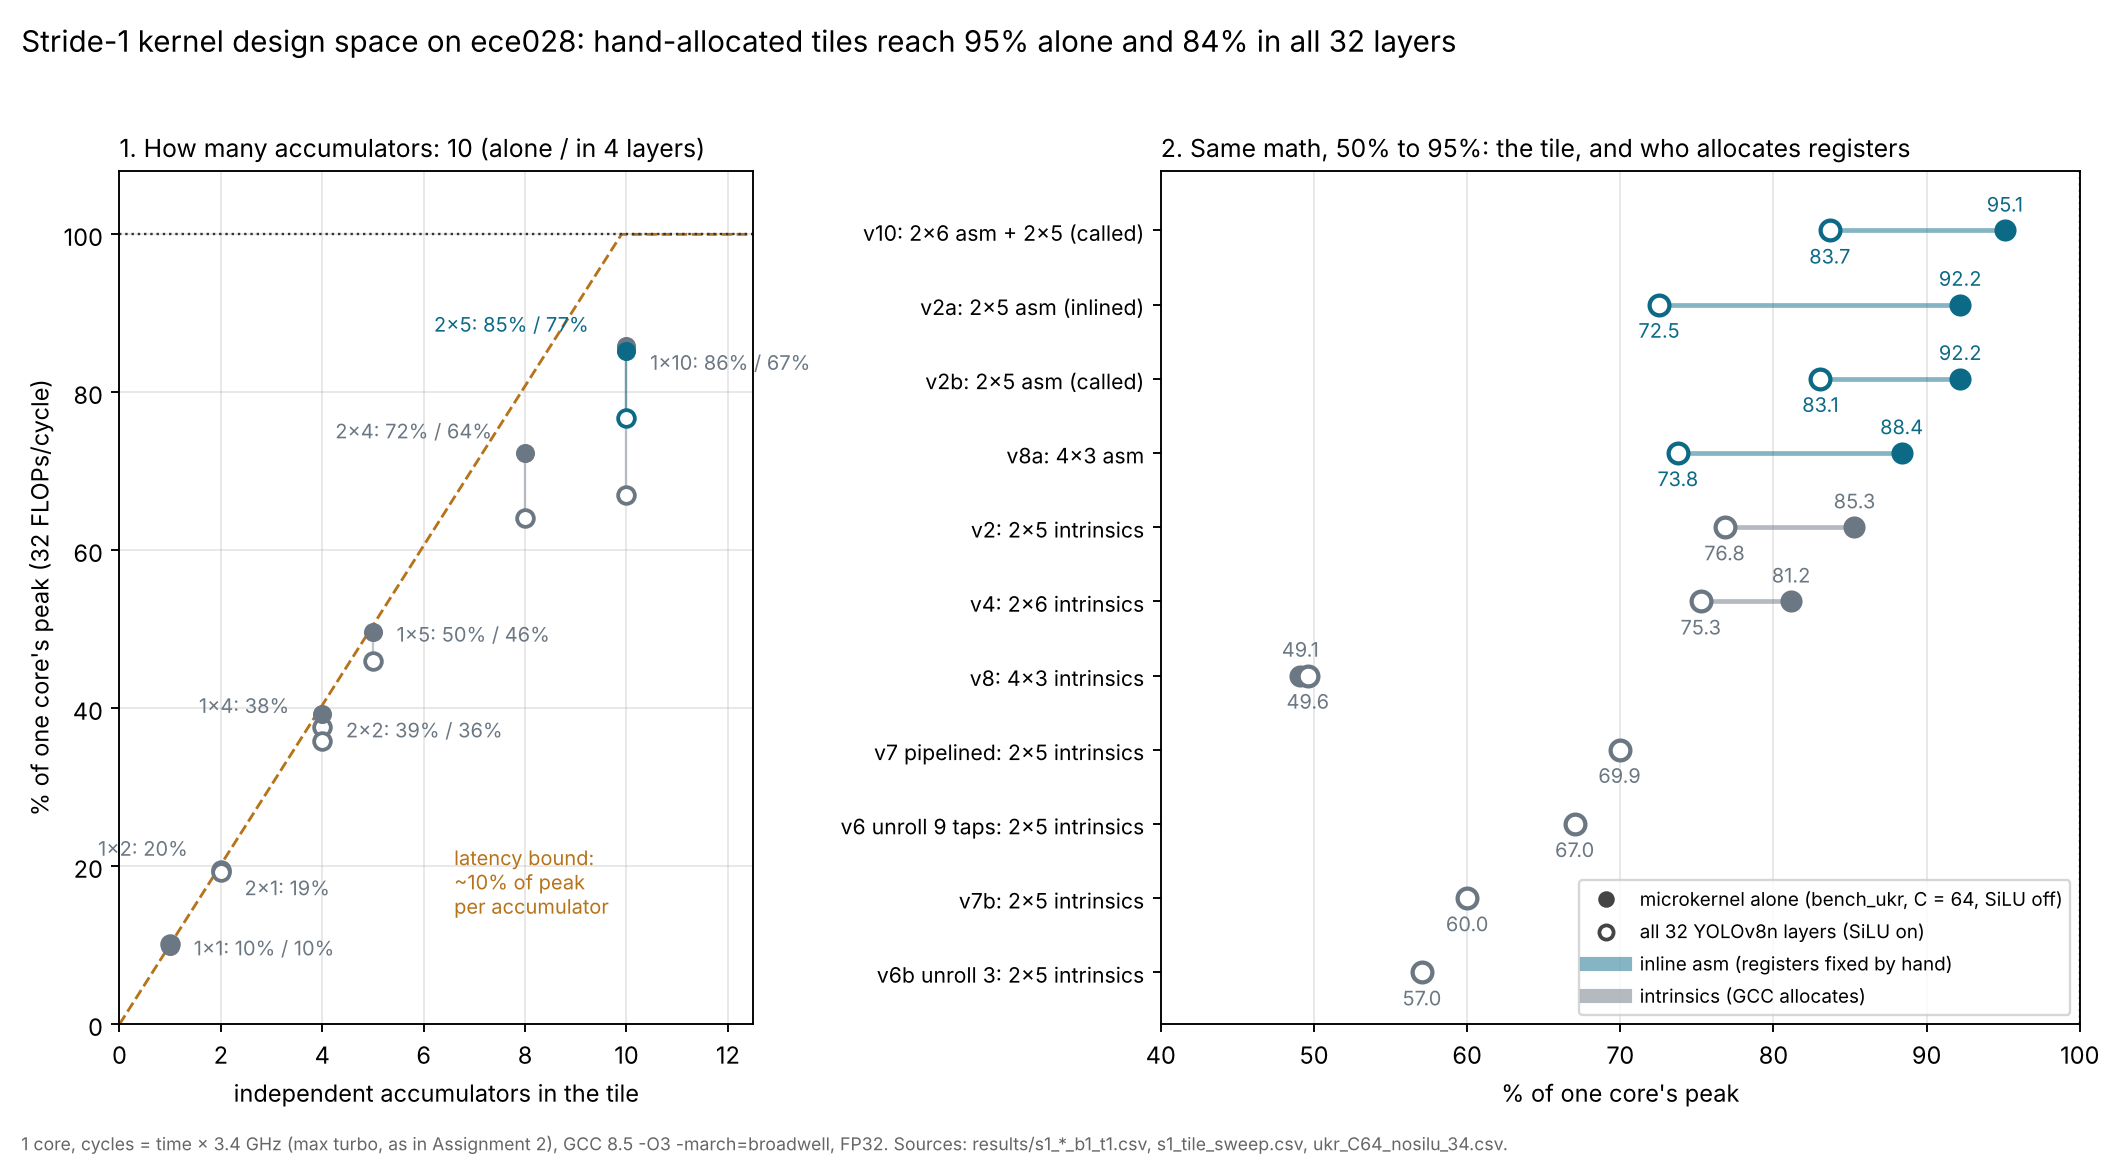
\includegraphics[width=0.97\linewidth]{figs/ukr_design_space.png}
    \end{column}
    \begin{column}{0.18\textwidth}
      \scriptsize
      \begin{block}{Intrinsics}GCC: clean at 13 regs, copies at 15, spills at 16\end{block}
      \begin{alertblock}{Inline asm}2$\times$6 by hand: 95\% alone, 84\% in layers\end{alertblock}
      \begin{block}{Unroll, pipeline}lost: uop cache, spills\end{block}
    \end{column}
  \end{columns}
\end{frame}
\note{Every kernel I built, same arithmetic, same layout. Filled dots: the microkernel alone; hollow: all 32 layers.
Right: the 2x6 tile loses with intrinsics because GCC adds 11 register copies per tap at 15 live registers,
but with the registers fixed in inline asm it is the best kernel, 95\% alone. 4x3 needs all 16 registers; GCC spills it to 49\%.
Unrolling and software pipelining made it worse: full unrolling overflowed the uop cache and partial unrolling made GCC spill.}

% ------------------------------------------------------------------ 6. sweep
\begin{frame}{Benchmarked like Assignment 2: FLOPs/cycle vs $k$}
  \begin{columns}[T]
    \begin{column}{0.7\textwidth}
      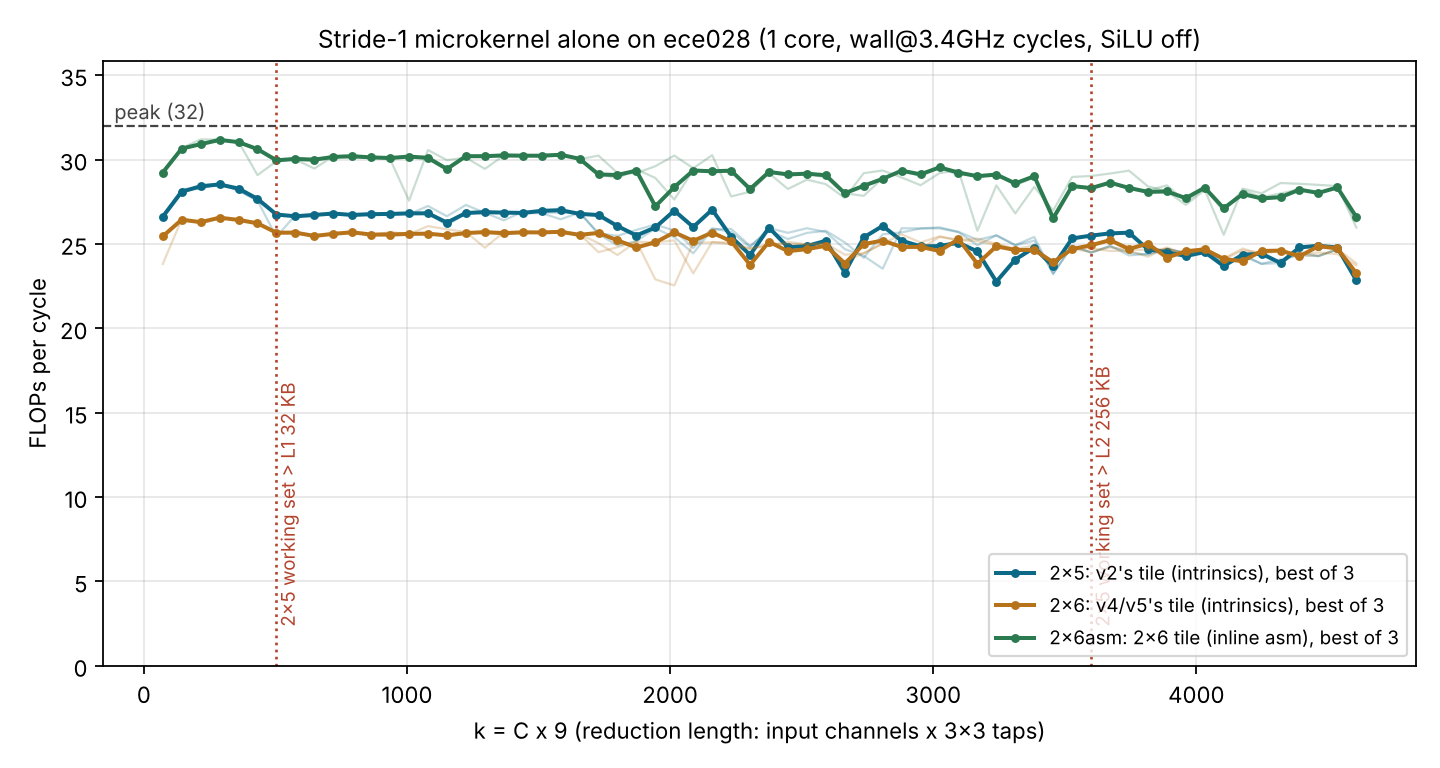
\includegraphics[width=\linewidth]{figs/ukr_sweep_nosilu_34.png}

      {\scriptsize\color{muted}SiLU off, cycles $=$ time $\times$ 3.4\,GHz, as in A2. 3 runs, every point checked (576 pass).}
    \end{column}
    \begin{column}{0.28\textwidth}
      \stat{94--97\%}{2$\times$6 asm: 30--31 FLOPs/cycle, $\sim$102 GFLOP/s on one core}\\[1.2em]
      \stat[grey]{83--89\%}{2$\times$5 intrinsics (v2's tile)}\\[1.2em]
      \stat[amber]{$k\approx500$}{L1 dip: 2$\times$5 weights pass 32\,KB, like $k\approx315$ in A2}
    \end{column}
  \end{columns}
\end{frame}
\note{This is the Assignment 2 figure for my kernel: FLOPs per cycle against the reduction length k.
Cycles are time times 3.4 GHz, the max turbo, exactly as in Assignment 2, so this can only understate.
2x6 asm holds 30 to 31 FLOPs per cycle, 94 to 97 percent of peak; 2x5 intrinsics 83 to 89.
The dip near k = 500 is the 2x5 weights leaving L1, like k = 315 in A2.
Cross-checked: the hardware FP-instruction counter matches our FLOP count exactly.}

% ------------------------------------------------------------------ 7. alone vs layers + baselines
\begin{frame}[fragile]{Alone vs in a layer: keep the kernel a function}
  \begin{columns}[T]
    \begin{column}{0.48\textwidth}
      \textbf{v2a (2$\times$5 asm): 92.2\% alone, 72.5\% when GCC inlines it into the layer loop}
      \vspace{0.4em}
\begin{semiverbatim}\footnotesize
vmovaps 168(%rsp), %ymm1   # reload acc
  ...asm block: 80 FMAs...
vmovaps %ymm1, 168(%rsp)   # store acc
\end{semiverbatim}
      {\small\color{muted}Inlined, GCC keeps 3 of 10 accumulators on the stack around every tap.
      Called as a function, as in the benchmark: 83.1\% (v2b); with the 2$\times$6 tile, 83.7\% (v10).}

      \vspace{0.8em}
      {\small\color{teal}\itshape Next: cache blocking for $C \geq 128$ (the 4$\times$3 drop-off), NUMA-aware threads (v10 on 20 cores: 4.74\,ms).}
    \end{column}
    \begin{column}{0.5\textwidth}
      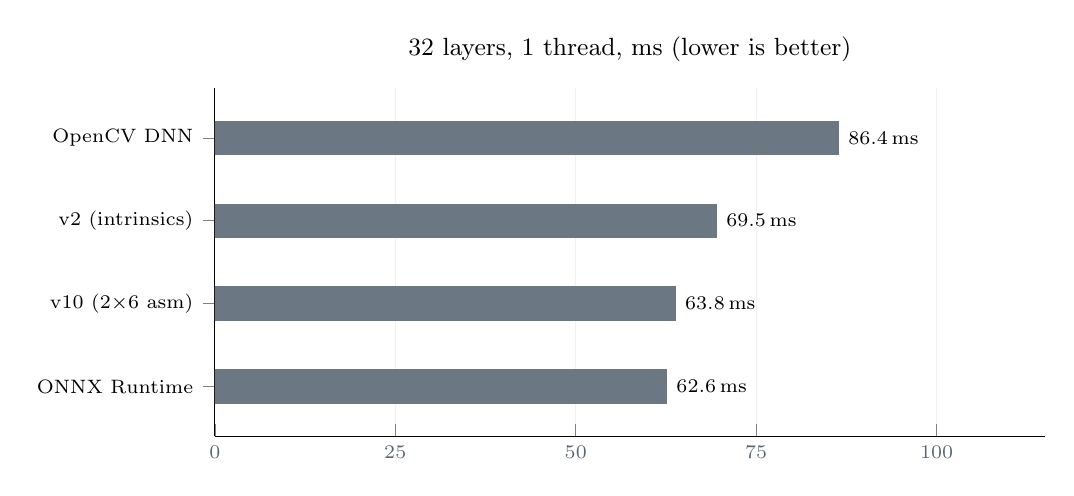
\begin{tikzpicture}
        \begin{axis}[width=\linewidth, height=6cm, xbar, bar width=12pt, xmin=0, xmax=115, xtick={0,25,50,75,100},
            symbolic y coords={ort,v10,v2,ocv}, ytick=data,
            yticklabels={ONNX Runtime,v10 (2$\times$6 asm),v2 (intrinsics),OpenCV DNN},
            y tick label style={font=\scriptsize}, x tick label style={font=\scriptsize, color=muted},
            nodes near coords={\pgfmathprintnumber[fixed,precision=1]{\pgfplotspointmeta}\,ms},
            nodes near coords style={font=\scriptsize}, axis lines*=left, xmajorgrids, grid style={color=soft},
            title={\small 32 layers, 1 thread, ms (lower is better)}, enlarge y limits=0.2]
          \addplot[fill=grey, draw=grey] coordinates {(62.6,ort) (63.8,v10) (69.5,v2) (86.4,ocv)};
        \end{axis}
      \end{tikzpicture}
    \end{column}
  \end{columns}
\end{frame}
\note{Kernel A, 2x5 in asm, beat kernel B, 2x5 intrinsics, by 7 points alone but lost by 4 in the layers.
The assembly shows why: inlined into the layer loop, GCC keeps 3 accumulators on the stack and reloads them around every tap.
Calling the microkernel as a function, exactly as the benchmark does, fixes it: 83.1\% for 2x5 and 83.7\% for v10, all at 3.4 GHz.
v10 is 1.36 times faster than OpenCV and within 2\% of ONNX Runtime on all 32 layers. Next: cache blocking and threading.}

% ------------------------------------------------------------------ backup
\begin{frame}{Backup: the same sweeps with SiLU on}
  \begin{columns}[T]
    \begin{column}{0.5\textwidth}
      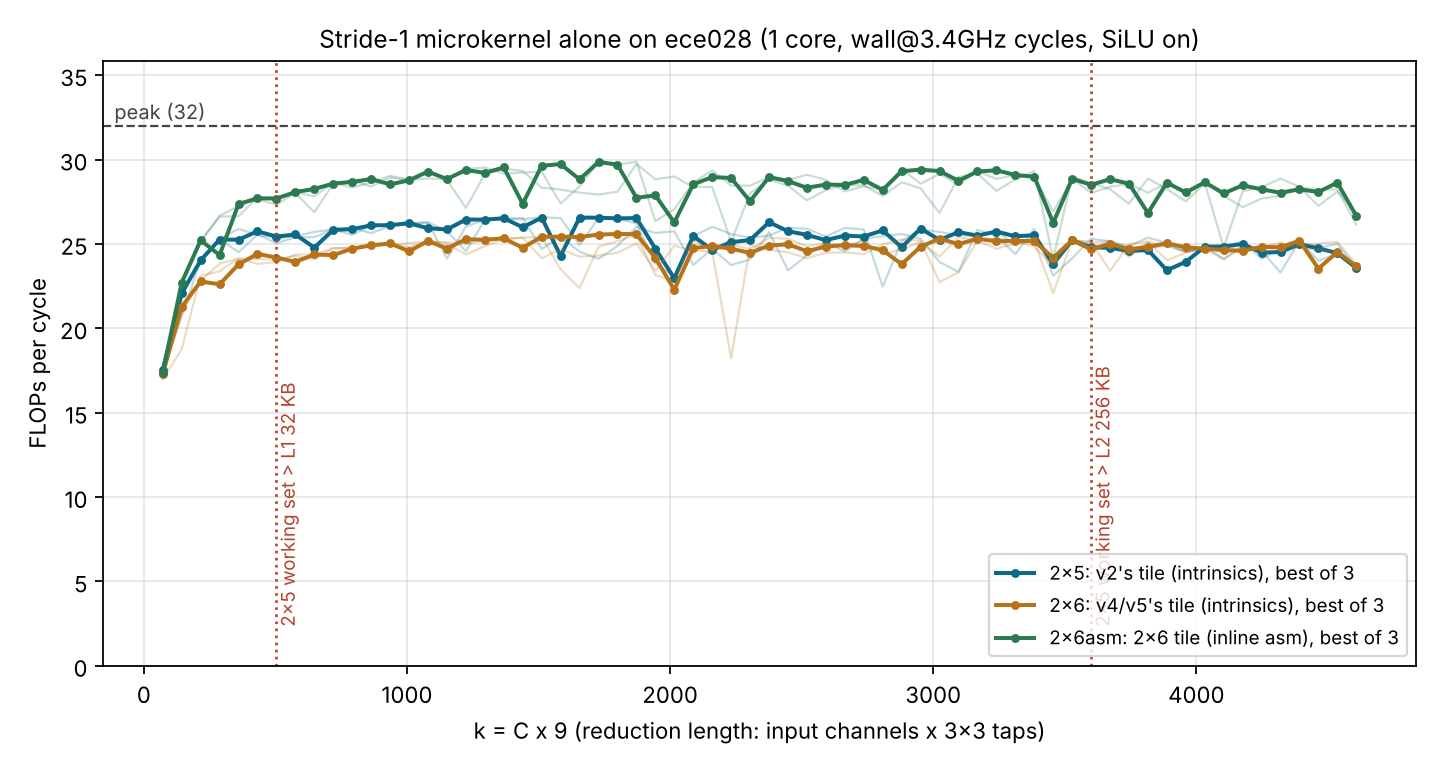
\includegraphics[width=\linewidth]{figs/ukr_sweep_2x6_34.png}

      {\scriptsize\color{muted}2$\times$6 asm 90.2\% mean ($C = 32$--256); 2$\times$5 81.4\%. SiLU costs a fixed 160--290 cycles per call.}
    \end{column}
    \begin{column}{0.5\textwidth}
      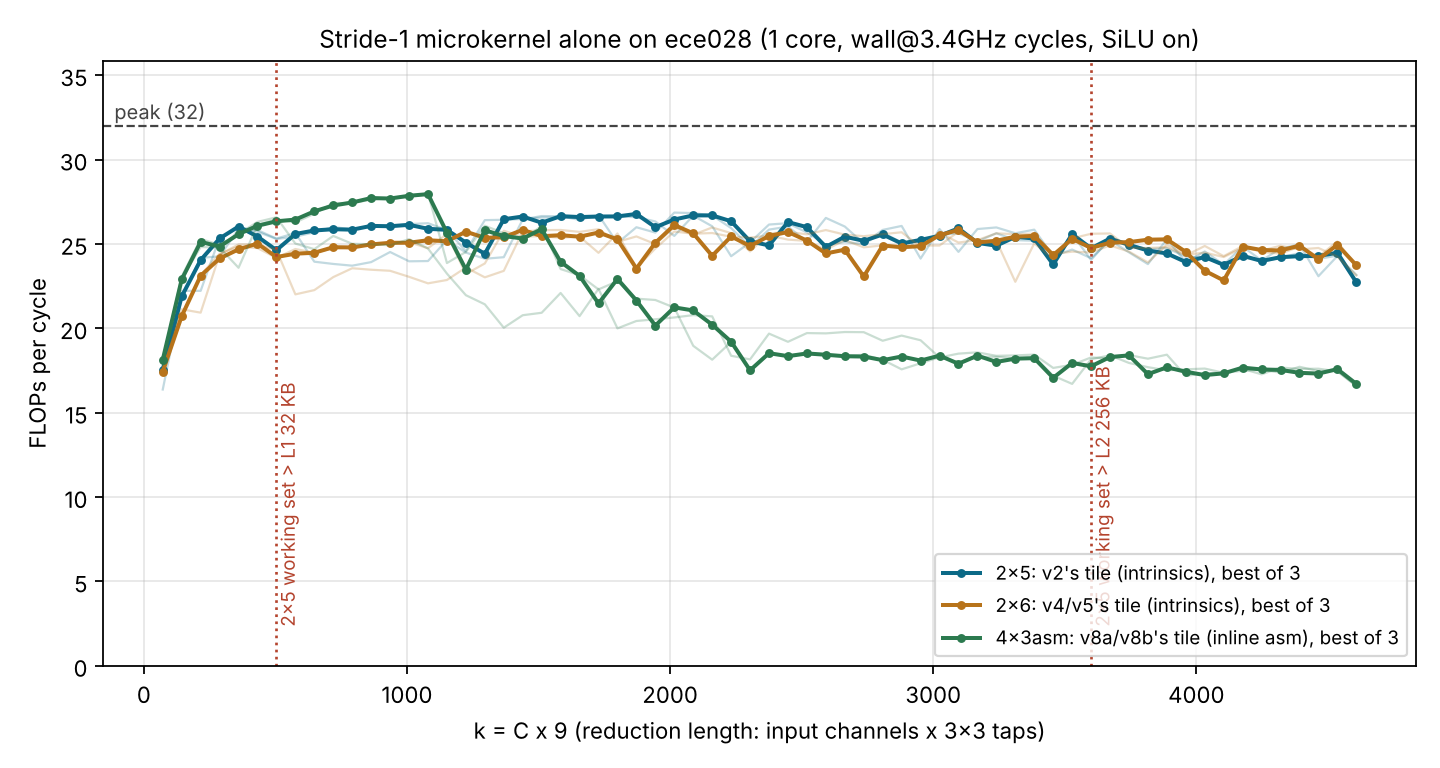
\includegraphics[width=\linewidth]{figs/ukr_sweep_34.png}

      {\scriptsize\color{muted}4$\times$3 asm: best 87.5\% at $C = 120$, 57\% at $C = 256$: its weights leave L2 (cache blocking fixes this).}
    \end{column}
  \end{columns}
\end{frame}

\end{document}
